\xchapter{Plano de Pesquisa}{}\label{plano}

\section{Considerações Iniciais}


%%%%sobre o projeto
%%%%falta uma definição formal do problema abordado

Este capítulo descreve como a pesquisa proposta neste mestrado será desenvolvida para permitir que medidas de similaridade (distância) sejam aplicadas para analisar séries temporais com ruído aditivo. Espera-se que com a análise individual dos componentes estocásticos e determinísticos, o agrupamento de séries temporais seja realizado com maior acurácia. A seguir, são apresentados detalhes sobre cada etapa do desenvolvimento do projeto.

\section{Descrição do problema}

Seja $X(t) = \{x_1, x_2, \dots, x_t\}$ uma série temporal univariada composta por $t$ observações. Suponha que $X(t)$ seja formada por um ruído aditivo onde cada observação de $X(t)$ é definida por $x_i = D_i + E_i + T_i$, tal que $1 \leq i \leq t$ e $D_i$, $E_i$ e $T_i$ representam influências dos componentes determinístico, estocástico e tendência, respectivamente.

Considerando que as influências destes componentes podem ser decompostas utilizando abordagens disponíveis na literatura~\cite{Araujo2013, Araujo2015}, este projeto de mestrado visa comprovar a hipótese que conjuntos de dados formados por séries temporais podem ser agrupados com maior acurácia quando medidas de similaridades (ou distância) são, individualmente, aplicadas sobre seus componentes estocásticos e determinísticos.

Neste contexto, um conjunto de dados temporais pode ser representado por $Y=\{X_{\alpha}(\beta)\}$, $\alpha = \{1, \dots, n\}$, tal que $n \in \mathbb{N}$ representa o número de séries temporais existentes na base de dados e $\beta \in \mathbb{N}$ representa o número de observações em cada série temporal. É importante destacar ainda que $n \geq 2$, uma vez que não faz sentido encontrar estruturas em bases que contém apenas uma observação. Além disso, o tamanho das observações ($\beta$) precisa ser suficiente para execução dos métodos de decomposição. Em análises empíricas, notou-se que é possível aplicar o método EMD em séries com ruído aditivo que contêm ao menos $10$ observações.

Para exemplificar a execução desta proposta de mestrado, considere um agrupamento particional do tipo \emph{hard} que visa dividir $Y$ em $k$ grupos, $C = \{C_1, C_2, \dots, C_k\}$, sendo $k \leq n$. Os grupos obtidos devem respeitar as seguintes restrições: i) $C_i$ $\neq \emptyset, 1 \leq i \leq k$; ii) $\bigcup_{i=1}^{k} C_i = Y$; e iii) $C_i \cap C_j = \emptyset$, $i,j = \{1, \dots, k\}$ e $i \neq j$.

Para determinar se duas séries devem pertencer a um mesmo grupo, utiliza-se medidas de similaridade ou distância ($\mathbb{D}$). Neste caso, para um conjunto de dados com $n$ séries temporais, uma matriz de similaridade $\mathbb{M}$ ($n\textbf{x}n$) pode ser construída calculando $\mathbb{M}_{p,q} = \mathbb{D}_{p,q}$.

Para exemplificar, considere duas séries temporais de mesmo tamanho $X_p(t)$ e $X_q(t)$. A distância entre essas séries pode ser calculada pela distância de Manhattan, $\mathbb{D}_{p,q} = \sum_{j=1}^{t} |X_p(j) - X_q(j)|$. Neste exemplo, considere que as tendências das séries foram removidas\footnote{Em geral, a tendência pode ser considerada como um comportamento determinístico, uma vez que sua influência em um dado instante depende apenas das tendências de instantes anteriores.}, sendo que suas observações são compostas apenas pelas influências estocásticas e determinísticas, i.e., $\mathbb{D}_{p,q} = \sum_{j=1}^{t} |(D_{p,j} + E_{p,j}) - (D_{q,j} + E_{q,j})|$. Logo, podemos reescrever o cálculo da distância pela Equação \ref{eq:decompDist}.

\begin{align}\label{eq:decompDist}
\mathbb{D}_{p,q}&=\sum_{j=1}^{t} |(D_{p,j} + E_{p,j}) - (D_{q,j} + E_{q,j})| \nonumber\\
       &=\sum_{j=1}^{t} |(D_{p,j} - D_{q,j}) + (E_{p,j} - E_{q,j})|\nonumber \\
       &=\sum_{j=1}^{t} |D_{p,j} - D_{q,j}| + \sum_{j=1}^{t} |E_{p,j} - E_{q,j}|.\qedhere
\end{align}


Portanto, pode-se afirmar que a distância\footnote{Em agrupamento de dados, pode-se utilizar tanto medidas de distância como medidas de similaridade. Dependendo do algoritmo utilizado, a distância pode ser obtida pelo inverso da similaridade.} entre duas séries com ruído aditivo pode ser calculada considerando individualmente as distâncias entre seus componentes estocásticos e determinísticos.

Assim, aplicando a decomposição em série temporais, espera-se construir uma matriz de similaridade $\mathbb{M}$  que pode ser utilizada por algoritmos de agrupamento, encontrando partições $C$ com maior acurácia.

%%%%

A Figura \ref{prop1} apresenta de maneira resumida a execução deste projeto. Para o cálculo da distância entre duas séries temporais $X_p(t)$ e $X_q(t)$, é realizada uma decomposição que extrai seus componentes estocásticos ($E_p$ e $E_q$, respectivamente) e determinísticos ($D_p$ e $D_q$, respectivamente).

\begin{figure}[!ht]
\begin{center}
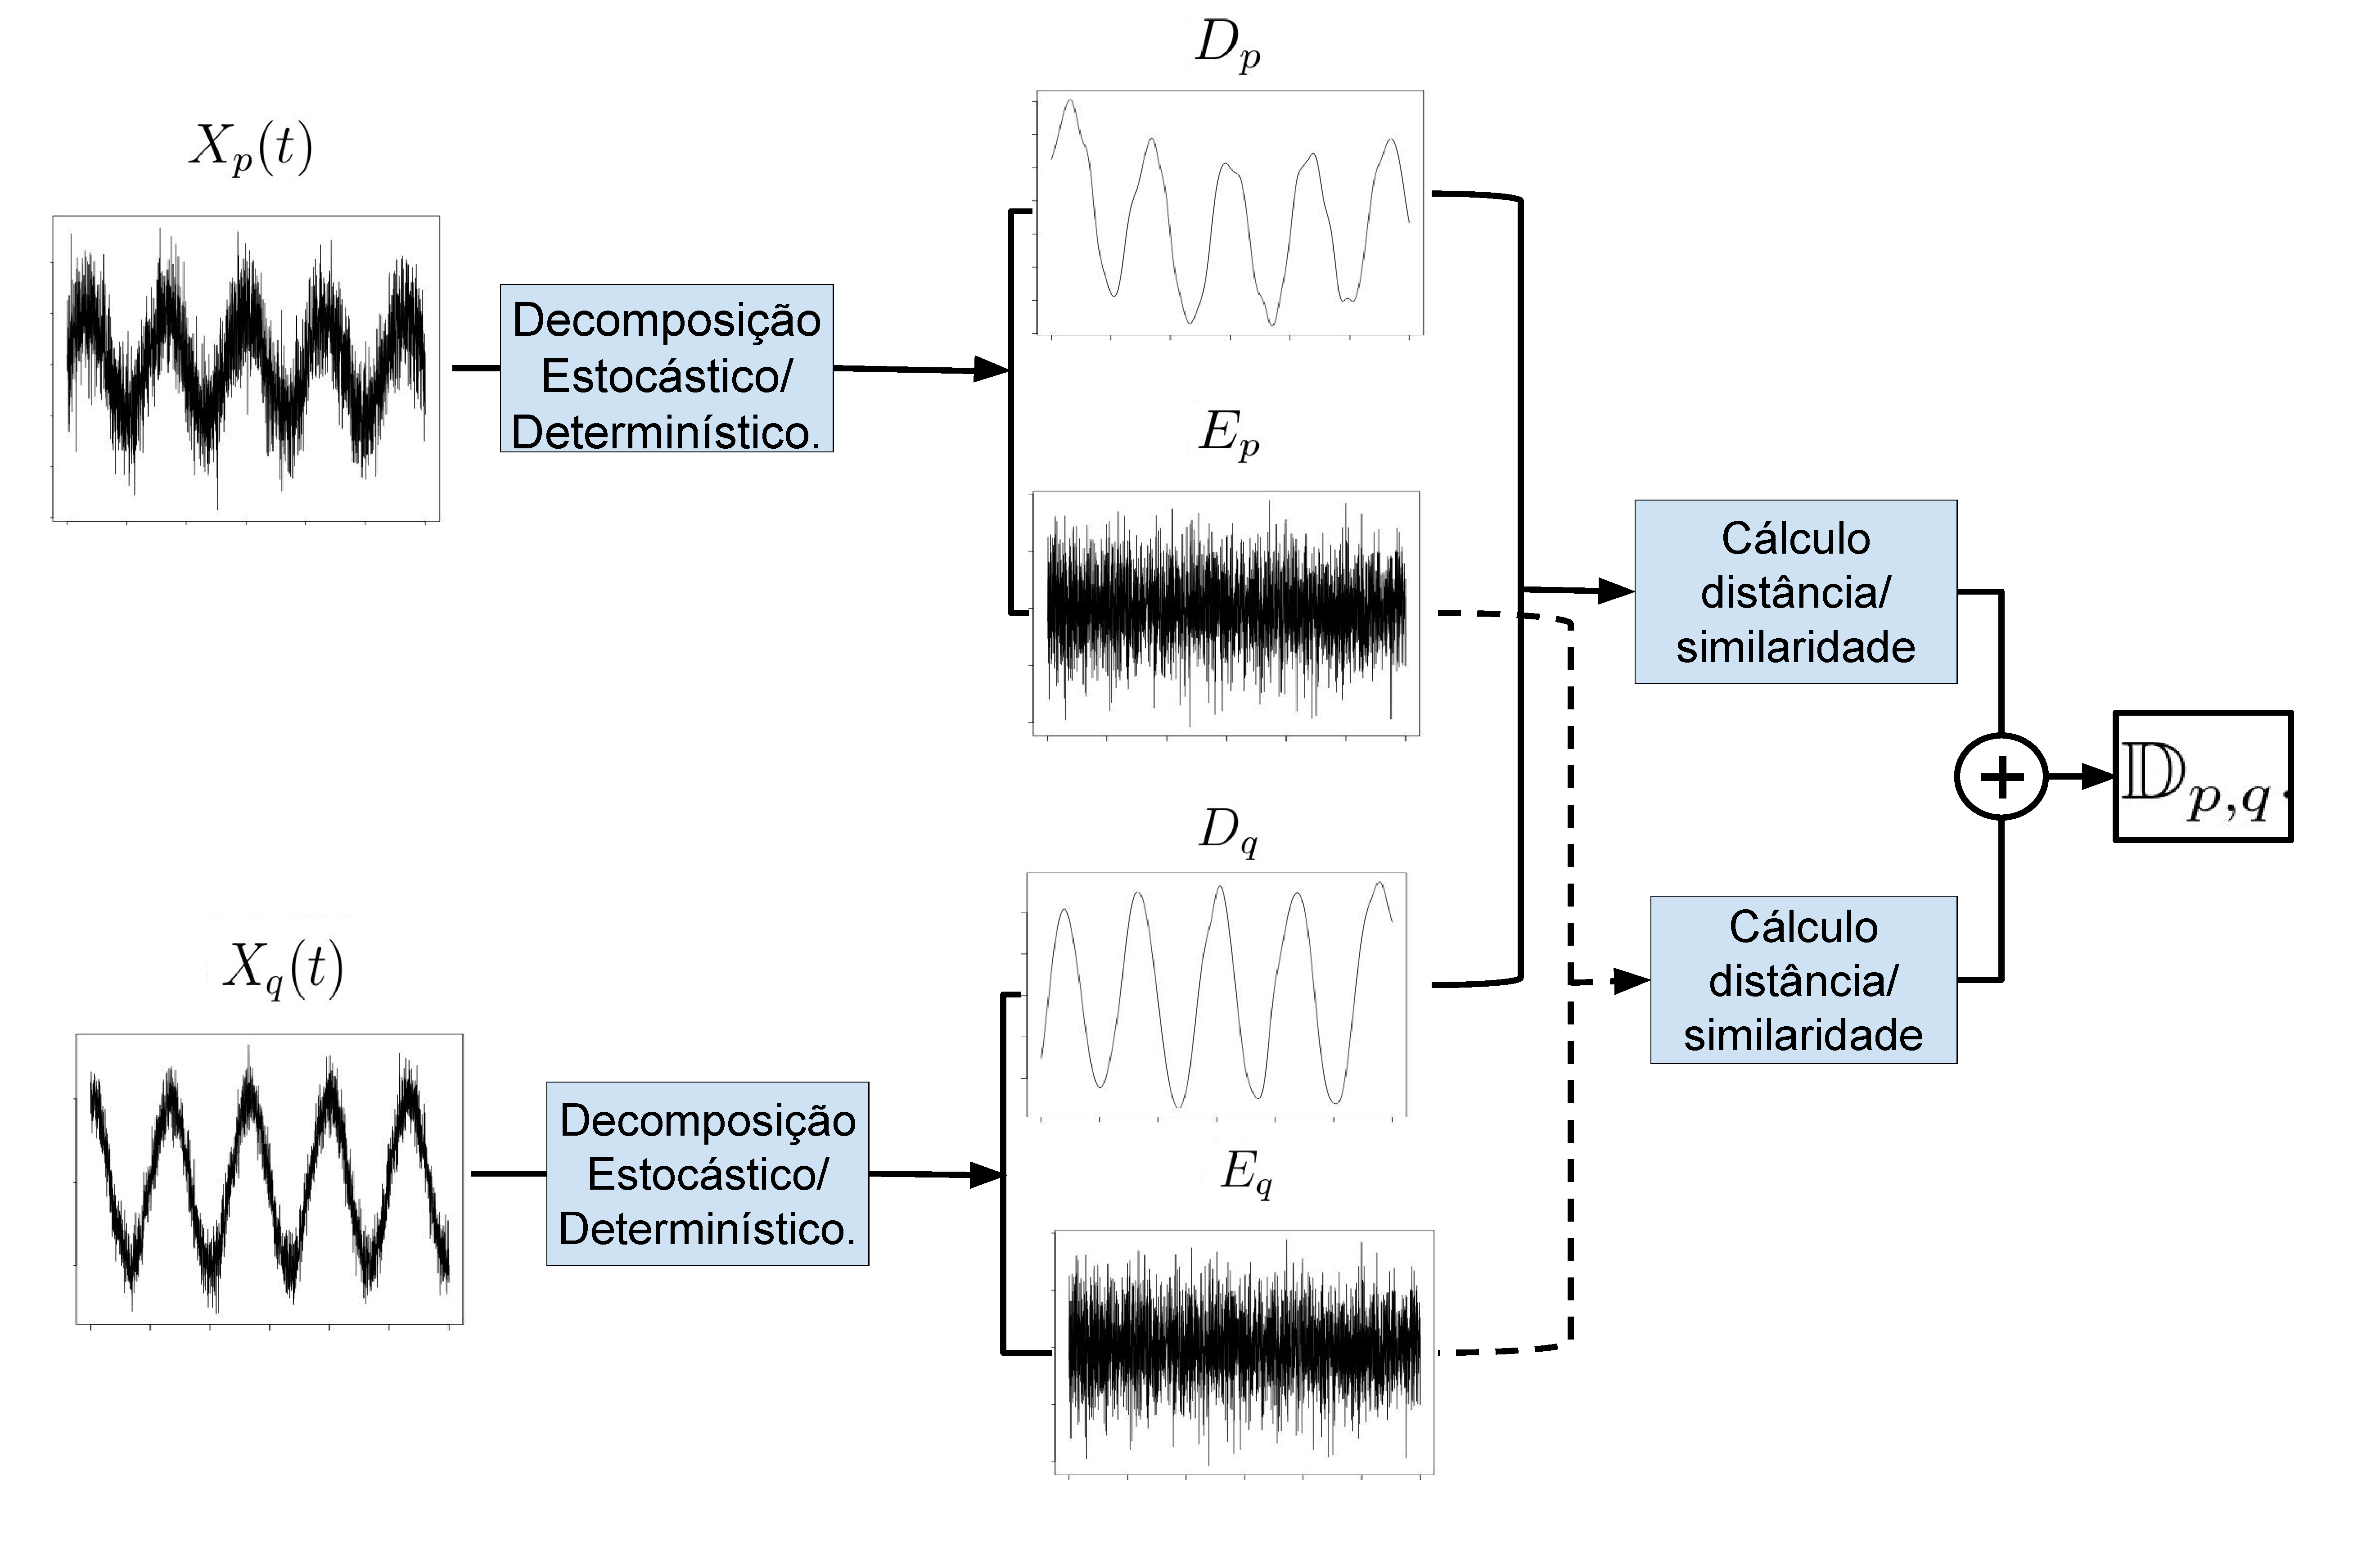
\includegraphics[scale=0.2]{esquema.pdf}
\caption{Proposta do projeto de mestrado.}
\label{prop1}
\end{center}
\end{figure}

Em seguida, aplica-se uma medida de distância de maneira isolada entre os componentes, ou seja, calcula-se a distância entre os componentes estocásticos da série e a distância entre os componentes determinísticos, reduzindo o impacto da presença de ruído nas medidas utilizadas. Por fim, a distância entre os componentes é combinada para formar a distância geral entre as séries originais $\mathbb{D}_{p,q}$.

Em contraste com trabalhos encontrados na literatura, ao realizar uma decomposição de séries temporais, torna-se viável combinar medidas de distância que fornecem bons resultados para séries estocásticas com medidas usualmente aplicadas sobre séries determinísticas. 

\subsection{Atividades da pesquisa}

A Tabela \ref{cronograma} apresenta o cronograma das atividades planejadas para a realização da pesquisa. Atividades concluídas são representadas pelo símbolo $X$ e as futuras por $\bullet$. 



\begin{table}[htbp]
\caption{Cronograma de atividades}     % mude aqui para seu título da tabela
\begin{center}
\resizebox{\textwidth}{!}{ % abre resizebox, setar tabela da largura da página.
\begin{tabular}{|c|l|l|l|l|l|l|l|l|l|l|l|l|l|l|l|l|l|l|l|l|l|l|l|l|}
\hline
\multicolumn{1}{|c|}{\multirow{2}{*}{Atividades}} & \multicolumn{24}{c|}{Meses} \\ \cline{2-25}
\multicolumn{1}{|c|}{} & 01 & 02 & 03 & 04 & 05 & 06 & 07 & 08 & 09 & 10 & 11 & 12 & 13 & 14 & 15 & 16 & 17 & 18 & 19 & 20 & 21 & 22 & 23 & 24 \\ \hline
%\rowcolor[HTML]{EFEFEF}


1-Disciplinas & X & X & X & X & X & X & X & X & X & X & X & X & $\bullet$ & $\bullet$ & ~ & ~ & ~ & ~ & ~ & ~ & ~ & ~ & ~ & ~ \\ \hline
2-Revisão da Literatura & X & X & X & X & X & X & X & ~ & ~ & ~ & ~ & ~ & ~ & ~ & ~ & ~ &  ~ & ~ & ~ & ~ & ~ & ~ & ~ & ~ \\ \hline
3-Experimentos  & ~ & ~ & ~ & ~ & ~ & ~ & ~ & X & X & X & ~  & ~  & $\bullet$ & $\bullet$ & $\bullet$ & $\bullet$ & ~ & ~ & ~ & ~ & ~ & ~ & ~ & ~ \\ \hline
4-Análise dos Resultados & ~ & ~ & ~ & ~ & ~ & ~ & ~ & ~ & ~ & X & ~ & ~ & ~  & ~  & $\bullet$ & $\bullet$ & $\bullet$ & $\bullet$ & ~ & ~ & ~ & ~ & ~ & ~ \\ \hline
5-Escrita da qualificação & ~ & ~ & ~ & ~ & ~ & ~ & ~ & X & X & X & X & ~ & ~ & ~ & ~ & ~ & ~ & ~ & ~ & ~ & ~ & ~ & ~ & ~ \\ \hline
6-Estágio docente & ~ & ~ & ~ & ~ & ~ & ~ & ~ & ~ & ~ & ~ & X & X & $\bullet$ & $\bullet$ & ~ & ~ & ~ & ~ & ~ & ~ & ~ & ~ & ~ & ~ \\ \hline
7-Pesquisa Orientada & ~ & ~ & ~ & ~ & ~ & ~ & ~ & ~ & ~ & ~ & X & X & $\bullet$ & $\bullet$ & $\bullet$ & $\bullet$ & $\bullet$ & $\bullet$ & $\bullet$ & $\bullet$ & $\bullet$ & $\bullet$ & $\bullet$ & $\bullet$ \\ \hline
8-Apresentação da qualificação & ~ & ~ & ~ & ~ & ~ & ~ & ~ & ~ & ~ & ~ & ~ & ~ & $\bullet$ & ~ & ~ & ~ & ~ & ~ & ~ & ~ & ~ & ~ & ~ & ~ \\ \hline
9-Escrita de artigos& ~ & ~ & ~ & ~ & ~ & ~ & ~ & ~ & ~ & ~ & ~ & ~ & $\bullet$  & ~ & ~ & ~ & ~ & $\bullet$ & ~ & ~ & ~ & ~ & $\bullet$ & ~ \\ \hline
10-Escrita da dissertação& ~ & ~ & ~ & ~ & ~ & ~ & ~ & X & X & X & X & ~ & ~ & ~ & $\bullet$ & $\bullet$ & $\bullet$ & $\bullet$ & $\bullet$ & $\bullet$ & $\bullet$ & $\bullet$ & $\bullet$ & $\bullet$ \\ \hline
11- Defesa da dissertação& ~ & ~ & ~ & ~ & ~ & ~ & ~ & ~ & ~ & ~ & ~ & ~ & ~ & ~ & ~ & ~ & ~ & ~ & ~ & ~ & ~ & ~ & ~ & $\bullet$ \\ \hline

\hline
\end{tabular}
} % fecha resizebox
\end{center}
\label{cronograma} % para referencia no texto.
\end{table}

Para a conclusão da atividade 1, o Programa de Pós-Graduação em Ciência da Computação (PGCOMP) da Universidade Federal da Bahia (UFBA) exige que um mestrado obtenha um total de 18 créditos em disciplinas. Nos semestres 2016.1 e 2016.2, foram obtidos 15 créditos ao cursar as disciplinas: MATE64 -- Seminários Científicos, MATE65 -- Fundamentos de Pesquisa em Ciência da Computação I, MATD74 --  Algoritmos e Grafos, MATD33 -- Tópicos em Inteligência Computacional III e  MATE70 -- Computação Ubíqua e Sensível ao Contexto. No semestre corrente, 2017.1, está sendo cursada a disciplina MATE32 -- Tópicos em Inteligência Computacional II, completando os 3 créditos restantes. 

A segunda atividade planejada neste cronograma foi realizada em parceria com o aluno de bacharelado em Ciência da Computação Evaldo Machado Moreira Junior. O objetivo da sua monografia foi entender como as métricas são influenciadas pela presença de ruídos. Neste trabalho, as principais medidas/métricas de similaridade/distância entre séries temporais utilizadas por pesquisas na área foram encontradas com a execução de uma Revisão Sistemática de Literatura (\emph{Systematic Literature Review} -- SLR). 

As atividades 3 e 4 do cronograma consistem na realização dos experimentos e análise dos resultados. Essas atividades foram divididas em duas partes. A primeira contém apenas experimentos preliminares que foram realizados para validar esta proposta de trabalho. Nesta parte, séries temporais sintéticas com ruído aditivo foram criadas e analisadas conforme apresentado no Capítulo \ref{experimentos} e Apêndice \ref{apendice1}. A segunda parte dos experimentos e suas análises serão realizadas após a qualificação.

%As séries sintéticas foram montadas com componentes estocásticos e determinísticos, em uma parte do conjunto das séries foi acrescida tendência. Para os componentes estocásticos, foram criadas diversas observações com desvio padrão entre 0.1 e 1.0. Através desse conjunto foram obtido os componentes estocásticos e determinísticos após a aplicação da técnica de decomposição proposta por \cite{Araujo2013, Araujo2015}. Com isso, foram calculadas a similaridade/distância entre os componentes determinísticos obtidos.  A fim de comparar os resultados obtidos com o resultado entre as séries determinísticas originais. 

%Nos experimentos futuros, ainda com a decomposição obtida do experimento inicial, serão calculados os componentes  estocásticos através da análise no dominínio da frequência. Também será realizada a coleta de dados temporais reais para a realização de experimentos em um ambiente real e análise de seus resultados. 


As atividades 5 e 8 estão relacionadas com o componente curricular MATD75 -- Exame de qualificação. A atividade 5 refere-se à escrita deste texto e as atividades 6 e 7 representam os componentes curriculares MATA32 -- Estágio Docente e MATA31 -- Pesquisa Orientada, respectivamente. Além disso, durante a execução destas tarefas foi realizada a prova de proficiência em inglês. A atividade 8 está relacionada à apresentação desta qualificação de mestrado.
 
A escrita de artigos, listada no item 9 do cronograma, será realizada com base nos resultados gerados com os experimentos (Atividades $3$ e $4$) e nas contribuições obtidas com a apresentação da qualificação. Por fim, como requisito para a defesa de dissertação, fica pendente a atividade MATE93 -– Defesa de Proposta de Mestrado, a qual se refere aos itens 10 e 11 da Tabela \ref{cronograma}. 

\section{Considerações Finais}

Neste capítulo, apresentou-se de maneira detalhada o projeto de pesquisa, o plano de atividades e o cronograma planejado para a conclusão do mestrado. A seguir, no próximo capítulo, foram discutidos os resultados preliminares realizados com o objetivo de analisar a viabilidade da proposta de mestrado.

